\documentclass[conference]{IEEEtran}
 
\bibliographystyle{IEEEtran}
\usepackage{amsmath,amsthm}
\usepackage{listings}
\usepackage{tikz}
\usepackage{subfigure}
\usepackage{multirow}
\usepackage{pgfplots}
\usepackage{booktabs}
\usepackage{dcolumn}
\usepackage{cancel}
\usepackage{graphics}
\usepackage{url}

\newcommand{\infrule}[2]{\displaystyle\frac{\displaystyle\strut{#1}}{\displaystyle\strut {#2}}}
\newcommand{\deref}{\ast}
\newcommand{\rread}[1]{\mbox{\em Read}(#1)}
\newcommand{\rwrite}[1]{\mbox{\em Write}(#1)}
\newcommand{\lca}[2]{#1 \sqcup #2}
\newcommand{\rleq}{\leq}
\newcommand{\interval}[1]{\mbox{\em interval}(#1)}
\newcommand{\context}[1]{\mbox{\em context}(#1)}
\newtheorem{theorem}{Theorem} 
\newtheorem{lemma}[theorem]{Lemma}
\newtheorem{observation}[theorem]{Observation}

\begin{document}

\pdfpagewidth=8.5in
\pdfpageheight=11in

\title{Legion: Expressing Locality and Independence with Logical Regions}
\author{
\IEEEauthorblockN{Michael Bauer\IEEEauthorrefmark{1},
%\authorinfo(Stanford University, email: \mbox{mebauer@cs.stanford.edu}
Sean Treichler\IEEEauthorrefmark{1}, 
%\authorinfo(Stanford University, email: \mbox{sjt@cs.stanford.edu}
Elliott Slaughter\IEEEauthorrefmark{1}, 
% \authorinfo(Stanford University, email: \mbox{slaughter@cs.stanford.edu}
Alex Aiken\IEEEauthorrefmark{1}  
%\authorinfo(Stanford University, email: \mbox{aiken@cs.stanford.edu}
%\email{aiken@cs.stanford.edu}
}
\IEEEauthorblockA{
\IEEEauthorrefmark{1}{Computer Science Department, Stanford University}
}
}

\maketitle


\begin{abstract}
Modern parallel architectures have both heterogeneous processors and
deep, complex memory hierarchies.  We present Legion, a programming
model and runtime system for achieving high performance on these
machines.  Legion is organized around {\em logical regions}, which
express both locality and independence of program data, and {\em
  tasks}, functions that perform computations on regions.  We describe
a runtime system that dynamically extracts parallelism from
Legion programs, using a distributed, parallel scheduling algorithm
that identifies both independent tasks and nested parallelism.  Legion
also enables explicit, programmer controlled movement of data through
the memory hierarchy and placement of tasks based on locality
information via a novel mapping interface.  We evaluate our Legion
implementation on three applications: fluid-flow on a regular grid,
a three-level AMR code solving a heat diffusion equation, and 
a circuit simulation.
%
% FIXME: put some performance numbers here
%
\end{abstract}

\section{Introduction}
\label{sect:intro}
%Put intro text here \cite{Fatahalian06}

Modern parallel machines are increasingly complex, with deep,
distributed memory hierarchies and heterogeneous processing units.  Because the
costs of communication within these architectures vary by several orders of magnitude, 
the penalty for mistakes in the placement of data or computation is usually very poor performance.  Thus,
to achieve good performance the programmer
and the programming system must reason about {\em locality} (data resident
close to computation that uses it) and {\em independence} (computations
operating on disjoint data, and therefore not requiring communication and able to be placed in possibly distant parts of the machine).  
Most contemporary
programming systems have no facilities for the programmer to express locality
and independence.  The few languages that do focus primarily on
array-based locality \cite{Fatahalian06,CHAPEL04,UPC99} and 
avoid irregular pointer data structures.  
%
% FIXME
% Sean would like a bit more on why other systems don't support pointer data structures (e.g., the difficulty of
% alias analysis.  I thought about it and feel it is too much of a digression: mentioning that in the first paragraph
% makes it sound like it will be an important part of the paper.
%
%encode such structures in arrays, which 
%data structures encoded in arrays which are impossible for compilers
%and runtime systems to reason about with regard to locality and independence.

In this paper we describe Legion, a parallel programming system based
on using {\em logical regions} to describe the organization of data
and to make explicit relationships useful for reasoning about locality
and independence.
A logical region names a set of objects.  Logical regions are first-class 
values in Legion and may be dynamically allocated, deleted and stored
in data structures. Regions can also be passed as arguments
to distinguished functions called {\em tasks} that access the data in
those regions, providing locality information.  Logical regions may be
{\em partitioned} into disjoint or aliased (overlapping) {\em subregions}, providing
information for determining independence of computations.
Furthermore, computations access logical regions with particular {\em
  privileges} ({\em read-only}, {\em read-write}, and {\em reduce}) and {\em coherence} (e.g., {\em exclusive access} and {\em
  atomic access}, among others).  Privileges express how a task may use
its region arguments, providing data dependence information that
is used to guide the extraction of parallelism.  For example, if two tasks
access the same region with read-only privileges the two tasks
can potentially be run in parallel.
Coherence properties express the required semantics of concurrent region accesses.
For example, if the program executes $f_1(r); f_2(r)$ and tasks $f_1$
and $f_2$ both require {\em exclusive} access to region $r$, then Legion guarantees the result will
be as if $f_1(r)$ completes before $f_2(r)$ begins.   On the other hand, if
the tasks access $r$ with {\em atomic} coherence, then Legion
guarantees only atomicity of the tasks with respect to $r$: either task $f_1(r)$
appears to run entirely before $f_2(r)$ or vice versa.

Logical regions do not commit to any particular layout of the data or
placement in the machine.  At runtime, each logical region has one or
more {\em physical instances} assigned to specific memories.  It is often useful to have multiple
physical instances of a logical region (e.g., to replicate read-only data, or to allow
independent reductions that are later combined).

To introduce the programming model, we present
a circuit simulation in
Section~\ref{sec:ex}, illustrating regions, tasks,
permissions and coherence properties, the interactions between them,
and how these building blocks are assembled into a Legion
program.  Subsequent sections each describe a contribution in the
implementation and evaluation of Legion:

\lstset{
  language=C++,
  basicstyle=\scriptsize,
  numbers=left,
  numberstyle=\tiny,
  stepnumber=1,
  escapechar=\#,
  keepspaces=true,
  morekeywords={region_relation,region,coloring,partition},
  deletekeywords=float,
}
\begin{lstlisting}[float]
struct Node<rn>    { Node<rn>@rn next;    float charge, capacitance; }
struct Wire<rn,rn2,rw> { Wire<rn,rn2,rw>@rw next; Node<rn2>@rn in_node, out_node; float current, ... ; }
region_relation Circuit {
  region< Node<r_all_nodes> >                r_all_nodes;
  region< Wire<r_all_nodes,r_all_wires> >    r_all_wires;
  Node<r_all_nodes>@r_all_nodes              first_node;
  Wire<r_all_nodes,r_all_wires>@r_all_wires  first_wire;
}
region_relation CircuitPiece<rn, rw> {
  region< Node<rn_pvt+rn_shr> >                    rn_pvt (< rn), rn_shr (< rn);
  region< Node<rn> >                               rn_ghost (< rn);
  region< Wire<rn_pvt+rn_shr+rn_ghost,rn,rw_pvt> > rw_pvt (< rw);
  Node<rn_pvt+rn_shr>@(rn_pvt+rn_shr)              first_node;
  Wire<rn_pvt+rn_shr+rn_ghost,rn,rw_pvt>@rw_pvt    first_wire;
};
void simulate_circuit(Circuit c) : RWE(c.r_all_nodes,c.r_all_wires)
{
  coloring<c.r_all_wires> wire_owner_map = ... ; // wires colored by which piece they're in
  partition<c.r_all_wires> p_wires = partition(c.r_all_wires, wire_owner_map);
  coloring<c.r_all_nodes> node_owner_map = ... ; // nodes colored by which piece they're in
  coloring<c.r_all_wires> node_nghbr_map = ... ; // nodes colored by which pieces they neigbor
  coloring<c.r_all_wires> node_privacy_map = ... ; // nodes colored: 0 = no neighbors, 1 = some neighbors
  partition<c.r_all_nodes> p_nodes_pvs = partition(c.r_all_nodes, node_privacy_map);
  partition<p_nodes_pvs[0]> p_pvt_nodes = partition(p_nodes_pvs[0], node_owner_map);
  partition<p_nodes_pvs[1]> p_shr_nodes = partition(p_nodes_pvs[1], node_owner_map);
  partition<p_nodes_pvs[1]> p_ghost_nodes = partition(p_nodes_pvs[1], node_nghbr_map);

  CircuitPiece<c.r_all_nodes,c.r_all_wires> pieces[MAX_PIECES];
  for(i = 0; i < MAX_PIECES; i++) 
    pieces[i] <- { rn_pvt = p_pvt_nodes[i], rn_shr = p_shr_nodes[i],
                   rn_ghost = p_ghost_nodes[i], rw_pvt = p_wires[i] };

  while(!done) {
    for(i = 0; i < MAX_PIECES; i++) spawn(calc_new_currents(pieces[i]));
    for(i = 0; i < MAX_PIECES; i++) spawn(distribute_charge(pieces[i]));
    for(i = 0; i < MAX_PIECES; i++) spawn(update_voltages(pieces[i]));
  }
}

void calc_new_currents(CircuitPiece<rn,rw> piece): RWE(piece.rw_pvt), ROE(piece.rn_pvt,piece.rn_shr,piece.rn_ghost) {
  // read info from nodes connected to each wire, update state of wire
}

void distribute_charge(CircuitPiece<rn,rw> piece): ROE(piece.rw_pvt), RdA(piece.rn_pvt,piece.rn_shr,piece.rn_ghost) {
  // current moving through wires redistributes charge between nodes
}

void update_voltages(CircuitPiece<rn,rw> piece): RWE(piece.rn_pvt,piece.rn_shr)
{
  // total charge added to a node causes changes in voltage
}
\end{lstlisting}

 
\begin{itemize}

\item We define a {\em software out-of-order processor}, or SOOP, for
  scheduling tasks with region arguments in a manner analogous to how
  out-of-order hardware schedulers process instructions with register
  arguments (Section~\ref{sec:soop}).  In addition to pipelining the execution of tasks over
  several stages, our SOOP is distributed across the machine and is
  also hierarchical and naturally extracts nested
  parallelism (because tasks may recursively spawn subtasks).


%\item We use a {\em deferred execution} model that extracts parallelism
%even from highly irregular, unbalanced computations.  Instead of blocking,
%an operation $o$ that cannot immediately execute because it is dependent
%on some other operation $o'$ waits on an event that occurs when $o'$ completes.
%Events can be created for the completion of any operation in Legion, and 
%the scheduler can build long chains of deferred operations.  In Section~\ref{sec:exp}
%we show that dataflow-like deferred execution gives us a significant performance improvement
%over bulk synchronous global synchronization primitives such as barriers.

\item Of central importance is how
tasks are assigned (or {\em mapped}) to processors and how physical instances of logical regions are
mapped to specific memory units (Section~\ref{sec:mapping}).  Often using
application-specific information results in better
mappings than a generic mapping strategy.  We describe
a {\em mapping interface} that allows programmers to give the SOOP a specification
of how to map tasks and regions for a specific application, or even part of an
application.  This mapping API is designed so that
any user-supplied mapping strategy can only affect the performance of applications,
not their correctness.  
%Thus, user mappings only affect the time and resources required
%to run the program and cannot change the program's output.


\item We present results of experiments on three applications:
  fluid-flow on a regular grid, a three-level AMR code solving a
  heat diffusion equation and a circuit simulation.
  We compare each application with the best reference
  versions on three different clusters of multicore processors with
  GPUs, including the Keeneland supercomputer \cite{Keeneland}.
%
% FIXME Give the same numbers as in the abstract.
%

\end{itemize}

\section{Example: Circuit Simulator}
\label{sec:ex}

Listing~\ref{lst:code_ex} shows code for an electrical
circuit simulation, which illustrates the core features of the Legion programming model.
The circuit simulation takes a collection of
of wires and nodes where wires meet.  
The simulation repeatedly updates
currents, distributes charges, and updates voltages for as many
time steps as the simulation demands.  We first
describe the partitioning of regions in Section~\ref{subsec:partitioning}
and then describe the data type declarations in Section~\ref{subsec:datatypes}.

\subsection{Regions and Partitions}
\label{subsec:partitioning}

Line 9 declares the main simulator function, which takes a {\tt
Circuit} to be simulated.  This function specifies the regions it 
accesses and the {\em privileges} and {\em coherence} it requires of those regions.
In this case, the {\tt RWE} annotation specifies that the function
accesses the regions {\tt c.r\_all\_nodes} and {\tt c.r\_all\_wires}
with read-write privileges and {\em exclusive} coherence (i.e., no other
function can access these two regions concurrently).  The simulation 
reads and writes all nodes and wires, and it must be done
with exclusive access to ensure correct results.  Privileges specify what
the function can do with the regions; coherence specifies what other
functions can do with the regions concurrently.  Functions that
declare their accessed regions, privileges, and coherence are called {\em tasks}
and are the unit of parallel execution in Legion.

Lines 15-21 are responsible for partitioning the circuit into {\tt MAX\_PIECES}
pieces that can be worked on in parallel.  To partition a region, we
provide a {\em coloring}, which is a relation between the elements
of a region and a set of colors.  A {\em partition} is an object which given
a coloring and a region $r$ contains for each color $c$ a {\em subregion} of $r$
containing all the elements of $r$ colored $c$.

Wires are simply partitioned in {\tt MAX\_PIECES} subregions (line 16).  
The nodes are first partitioned into 
{\em private} and {\em shared} nodes (line 21).  Private nodes
are touched by a single task in a phase, while shared nodes may
be referenced by multiple tasks in a phase.  The thick lines in Figure~\ref{sfig:part_fig:pvs}
show how the nodes in a small graph might be partitioned into three subsets.  Gray
nodes are shared and black nodes are private.  Note that
this partition is disjoint since each node has one color.
%Our current implementation uses small
%integers or booleans for the names of colors, but any enumerable set would be
%fine.  The coloring relation need not be total - it can leave out some elements entirely.  And although it is not required to be injective (it can map a single
%element to multiple colors), the fact that injective mappings will always
%result in disjoint subregions makes them strongly encouraged (when possible).
%Our example uses four colorings to create circuit partitions.

We next further partition the private and shared subregions into {\tt
  MAX\_PIECES} disjoint subregions each (lines 20-23); one subregion
of the private and shared node partitions is shown in
Figures~\ref{sfig:part_fig:p_i} and \ref{sfig:part_fig:s_i}
respectively.  

We partition the shared nodes a second time using a
different coloring into the sets of ghost nodes for each task.  This 
partition is noteworthy because the subregions are not disjoint:
ghost nodes may be read by multiple tasks, and thus a node $n$  may belong 
to more than one ghost region, which corresponds to $n$ being assigned
more than one color by the coloring {\tt node\_neighbor\_map}.
One of the ghost subregions is shown in Figure~\ref{sfig:part_fig:g_i}.

Figure~\ref{sfig:part_fig:tree} shows the final hierarchy of node
partitions;  the $*$ symbol indicates a partition is disjoint. This
{\em region tree} data structure plays an important role in scheduling
tasks for out-of-order execution (see Section~\ref{sec:soop}).


%(These subsets are hopefully reasonably compact, but the correctness
%of the simulation is not dependent on that.)  
%Once the subsets are known, the \emph{node\_owner\_map} is created by assigning
%each node the color corresponding to its subset.  The 
%\emph{wire\_owner\_map} assigns each wire to the same subset as its ``in\_node''.
%The \emph{node\_nghbr\_map} maps a node to color(s) of all wires that 
%connect to it.  Finally, the \emph{node\_sharing\_map} is derived from the
%\emph{node\_nghbr\_map}, with a node colored ``true'' if any colors other than 
%its own were used, and ``false'' if the only wires that connect to a node are
%in the same piece.
%Figure~\ref{fig:part_fig} shows how the partitions are defined.

%Line 19 uses the \emph{wire\_owner\_map} to partition the wires region of the
%circuit into a subregion for each piece, but the partitioning of the nodes is
%more complicated due to the sharing that is necessary between the pieces.
%First, the \emph{node\_sharing\_map} is used to create two subregions: $p\_nodes\_pvs[false]$ contains all the nodes that are private to some piece (i.e. will
%never be needed for the computations in any other piece), while $p\_nodes\_pvs[true]$ contains nodes that will be accessed by multiple pieces' computations.
%Each of these subregions is then partitioned using the $node\_owner\_map$ to
%create the subregions owned by each computation.  These are the $p_i$ and $s_i$
%subregions, shown in Figures \ref{sfig:part_fig:p_i} and \ref{sfig:part_fig:s_i}.  Finally, the $g_i$ subregions (shown in Figure~\ref{sfig:part_fig:g_i}) are
%created using the $node\_nghbr\_map$ to 
%create subregions that include the ``ghost'' nodes needed to perform each
%piece's calculations.

%With the partitioning operations completed, the various subregions are
%recorded in an array of {\tt CircuitPiece} structures.  Lines 32-33 fill in multiple
%fields of a {\tt CircuitPiece} at once.  The need for such a statement will be described in detail in 
%section \ref{subsec:datatypes}.

%Because a region relationship can have
%fields with types that refer its own fields' values, it is often not possible
%to assign fields one at a time without violating the type checking rules.
%The simultaneous assignment operator asks the type checker only to make sure
%that the fields in the structure would have the right (self-referential) types
%after all the fields have been changed.

Lines 31-57 form the bulk of the actual simulation, performing three passes
over the circuit in each iteration.  Each pass loops over an array of pieces (constructed on lines 27-30 from the partitions),
spawning a task for each piece.   There are no explicit requests for
parallel execution (the default semantics of {\tt spawn} is sequential 
execution of the spawned tasks) nor is there synchronization required between the
passes.  Both the fact that the tasks can be run in parallel within a pass
and the required inter-pass dependencies are determined automatically
by the Legion runtime based on the region access annotations on the task declarations
(see Section~\ref{sec:soop}).

%The declarations for the three subtasks are shown on lines 42-51.  
The  {\tt calc\_new\_currents} task reads and writes the wires subregion, 
the nodes subregion, and the ghost node region for its piece.
The {\tt distribute\_charge} subtask is a different phase that reads the piece's 
wires subregion and updates all nodes those wires touch.  However,
rather than requesting the ability to read and write the nodes (which would
require serialization of these tasks for correctness), the task declares that
it will use reorderable {\em reduction} operations and that the coherence requirement
is {\em atomic} rather than exclusive access. The final task is 
{\tt update\_voltages}, which writes the shared and private nodes for a piece
and reads the results of the previous task's reductions.

  
%Since the wire subregions are known to be disjoint,
%the write sets of invocations of $calc\_new\_currents$ do not overlap, and can
%therefore be safely run in parallel.


%As long as the
%runtime can guarantee to apply the reductions from multiple subtasks safely, it
%can run the subtasks themselves in parallel.  Each invocation of 
%$distribute\_charge$ will be delayed until the corresponding invocation of 
%$calc\_new\_currents$ has completed due to the read-after-write dependency on
%the corresponding wire subregion.  However, despite the apparent 
%write-after-read anti-dependency on the ghost node regions, $distribute\_charge$
%tasks will generally not have to wait on the the completion of the other
%$calc\_new\_current$ tasks.  If there is sufficient memory available to make
%two copies of those nodes, the runtime can allow $distribute\_charge$ tasks to
%start calculating a new version of the nodes while older $calc\_new\_currents$
%tasks are still referring to the older version, all completely transparently to
%the application code.

%Again, the disjointness of the $p_i$ and $s_i$
%node subregions allows the runtime to safely run these tasks in parallel.  In
%this case, the runtime does wait for the completion of all the tasks in the 
%previous pass.  The read-after-write dependence on the $p_i$ is a guaranteed
%conflict, but there is also potential overlap between the $s_i$ subregions
%being reduced to in the previous pass and the $g_i$ subregions being accessed
%in this pass.  Although not every pair of $s_i$ and $g_j$ conflict, the
%runtime knows that they were created from two independent partitioning
%operations and guarantees correctness by conservatively assuming they might
%conflict.


\subsection{Data Types}
\label{subsec:datatypes}
The two basic data types in the circuit simulation are {\tt Node}s and
{\tt Wire}s declared on lines 1 and 2 of Listing~\ref{lst:code_ex}.
As is standard in region-based systems, allocating a {\tt Node}, {\tt
  Wire}, or any value in the heap requires naming the logical region
in which the value is allocated.  For example, {\tt new Node@r} returns
a reference to a new value of {\tt Node} type in region {\tt r}.  
Listing~\ref{lst:code_ex} illustrates one way of constructing partitioned
data structures in Legion: populate a region with data (using {\tt new}) and then partition it
into subregions.  Legion also supports partitioning an empty region into subregions
and then allocating data in the subregions; we use both approaches in our
application discussed in Section~\ref{sec:ex}.


Pointers to region values declare the region to which they point.  For
example, the definition of {\tt Wire} is parameterized on the region
{\tt rn} to which the {\tt Node} pointers in fields {\tt in\_nodes}
and {\tt out\_nodes} point, which guarantees that the two endpoints of
a wire are always in the same region.

Regions are first-class values in Legion and can be stored in heap
data structures.  For example, a {\tt Circuit} (defined on line 3)
holds the regions hold all nodes and wires of the circuit and a {\tt
  CircuitPiece} (defined on line 4) hold pointers to the private,
shared, and ghost nodes as well as the private wires of its piece of
the circuit.





%\def\partitiontree{
%\draw[step=0.5,gray,very thin] (0,0) grid (8,5);

\node(top) at (3.5,4.5) { $r{\_}all{\_}nodes$ };

\node(pvsf) at (1.9,2.5) { $p{\_}nodes{\_}pvs[0]$ };
\node(pvst) at (5.1,2.5) { $p{\_}nodes{\_}pvs[1]$ };

\node(p0) at (0.7,0.5) { $p_0$ };
\node(p1) at (1.2,0.5) { $p_1$ };
\node(pd) at (1.6,0.5) { $\ldots$ };
\node(pn) at (2.3,0.5) { $p_{n-1}$ };

\node(s0) at (3.2,0.5) { $s_0$ };
\node(s1) at (3.7,0.5) { $s_1$ };
\node(sd) at (4.1,0.5) { $\ldots$ };
\node(sn) at (4.8,0.5) { $s_{n-1}$ };

\node(g0) at (5.7,0.5) { $g_0$ };
\node(g1) at (6.2,0.5) { $g_1$ };
\node(gd) at (6.6,0.5) { $\ldots$ };
\node(gn) at (7.3,0.5) { $g_{n-1}$ };

\draw[xshift=3.5cm,yshift=3.5cm] (-1,0) -- (1,0)
  node(ptf)[pos=0.25,inner sep=0] {} edge (pvsf.north)
  node[pos=0.5,anchor=south east] {$*$}
  node(ptp)[pos=0.5,inner sep=0] {} edge (top.south)
  node(ptt)[pos=0.75,inner sep=0] {} edge (pvst.north)
  ;

\draw[xshift=1.5cm,yshift=1.5cm] (-1,0) -- (1,0)
  node(pp0)[pos=0.2,inner sep=0] {} edge (p0.north)
  node(pp1)[pos=0.4,inner sep=0] {} edge (p1.north)
  node[pos=0.5,anchor=south east] {$*$}
  node(ppp)[pos=0.5,inner sep=0] {} edge (pvsf.250)
  node(ppn)[pos=0.8,inner sep=0] {} edge (pn.north)
  ;

\draw[xshift=4cm,yshift=1.5cm] (-1,0) -- (1,0)
  node(ps0)[pos=0.2,inner sep=0] {} edge (s0.north)
  node(ps1)[pos=0.4,inner sep=0] {} edge (s1.north)
  node[pos=0.5,anchor=south east] {$*$}
  node(psp)[pos=0.5,inner sep=0] {} edge (pvst.230)
  node(psn)[pos=0.8,inner sep=0] {} edge (sn.north)
  ;

\draw[xshift=6.5cm,yshift=1.5cm] (-1,0) -- (1,0)
  node(pg0)[pos=0.2,inner sep=0] {} edge (g0.north)
  node(pg1)[pos=0.4,inner sep=0] {} edge (g1.north)
  node[pos=0.5,anchor=south east] {}
  node(pgp)[pos=0.5,inner sep=0] {} edge (pvst.310)
  node(pgn)[pos=0.8,inner sep=0] {} edge (gn.north)
  ;
}

\def\partitiongraph{
%\draw[step=0.5,gray,very thin] (0,0) grid (8,5);

\node[cn,s0] (n1) at (0.77,1.27) {};
\node[cn,p0] (n2) at (1.6165,3.3865) {};
\node[cn,s0] (n3) at (2.463,2.54) {};
\node[cn,p0] (n4) at (0.8755,2.54) {};
\node[cn,p2] (n5) at (2.463,0.529) {};
\node[cn,s2] (n6) at (3.945,1.799) {};
\node[cn,s0] (n7) at (3.6275,2.963) {};
\node[cn,p2] (n8) at (4.7915,0.529) {};
\node[cn,s1] (n9) at (5.638,1.5875) {};
\node[cn,s1] (n10) at (6.6965,1.164) {};
\node[cn,s1] (n11) at (5.215,2.6455) {};
\node[cn,p1] (n12) at (6.379,2.7515) {};
\node[cn,p1] (n13) at (5.3205,3.598) {};
\node[cn,s1,g0] (n14) at (4.1565,4.1275) {};
\node[cn,s0] (n15) at (2.8865,3.81) {};
\node[cn,p0] (n16) at (0.77,4.1275) {};
\node[cn,s2,g0] (n17) at (1.405,0.423) {};
\node[cn,p1] (n18) at (6.379,4.0215) {};
\node[cn,s2,g0] (n19) at (2.7805,1.4815) {};
\node[cn,s0] (n20) at (1.7225,1.799) {};
\node[cn,p2] (n21) at (3.733,0.7405) {};
\node[cn,s2] (n22) at (5.85,0.635) {};

\draw (n16) to (n2);
\draw (n16) to (n4);
\draw (n5) to (n21);
\draw (n21) to (n8);
\draw (n12) to (n13) to (n18) to (n12);


\draw[p2s] (n1) to (n4) to (n20);
\draw[p2s] (n4) to (n3) to (n15) to (n2);
\draw[p2s] (n15) to (n7);

\draw[p2s] (n14) to (n13) to (n11) to (n9) to (n12) to (n10);

\draw[p2s] (n17) to (n19) to (n5);
\draw[p2s] (n19) to (n6) to (n8) to (n22);

\draw[s2s] (n1) to (n17);
\draw[s2s] (n20) to (n19) to (n3);
\draw[s2s] (n15) to (n14) to (n7);
\draw[s2s] (n11) to (n6) to (n9) to (n22) to (n10);

\draw[thick] (0.5,0.5) to (4,2.5);
\draw[thick] (3.75,4.5) to (4,2.5);
\draw[thick] (6.5,0.5) to (4,2.5);

\draw[dashed] (0.5,1.5) .. controls (1,2) and (1.5,2.5) .. (1.9,3.1) .. controls (2,4) .. (1.75,4.5);
\draw[dashed] (5.25,4.5) .. controls (4.75,3.5) .. (5.25,3.25) .. controls (6,3) .. (6,2.5) .. controls (6,2.25) .. (7,2.5);
\draw[dashed] (2,0.25) .. controls (2.25,1) .. (3.5,1.1) .. controls (5,1.25) .. (5.5,0.25);
}

\begin{figure}[t]
  \centering
\subfigure[Node region tree.]{
\label{sfig:part_fig:tree}
%\begin{tikzpicture}[scale=0.8]
%\partitiontree
%\end{tikzpicture}
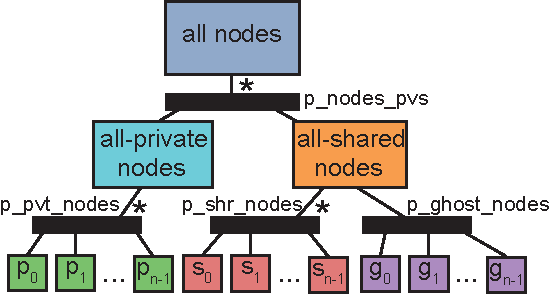
\includegraphics[scale=0.48]{figs/CircuitPartition.pdf}
}

  \subfigure[$p\_nodes\_pvs$]{
\label{sfig:part_fig:pvs}
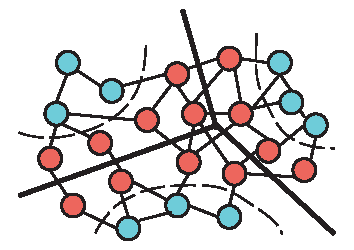
\includegraphics[scale=0.67]{figs/Private_vs_Shared.pdf}
}
  \subfigure[$p_i$]{
\label{sfig:part_fig:p_i}
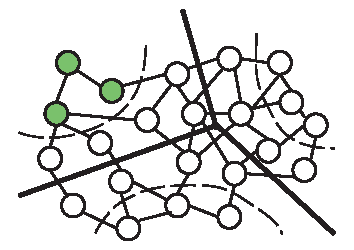
\includegraphics[scale=0.67]{figs/Private_Local.pdf}
}
  \subfigure[$s_i$]{
\label{sfig:part_fig:s_i}
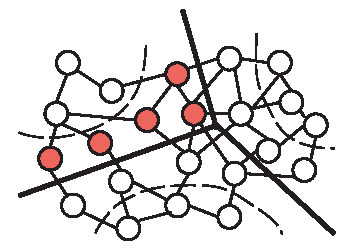
\includegraphics[scale=0.67]{figs/Shared_Local.pdf}
}
  \subfigure[$g_i$]{
\label{sfig:part_fig:g_i}
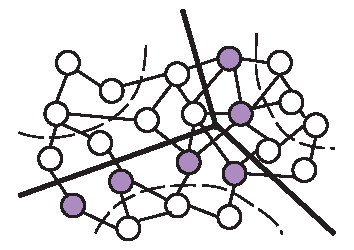
\includegraphics[scale=0.67]{figs/Ghost_Local.pdf}
}
  \label{fig:part_fig}
  \caption{Partitions of $r{\_}all{\_}nodes$.}
%  \caption[My caption
\end{figure}


%\lstset{
  language=C++,
  basicstyle=\scriptsize,
  numbers=left,
  numberstyle=\tiny,
  stepnumber=1,
  escapechar=\#,
  keepspaces=true,
  morekeywords={region_relation,region,coloring,partition},
  deletekeywords=float,
}
\begin{lstlisting}[float]
struct Node<rn>    { Node<rn>@rn next;    float charge, capacitance; }
struct Wire<rn,rn2,rw> { Wire<rn,rn2,rw>@rw next; Node<rn2>@rn in_node, out_node; float current, ... ; }
region_relation Circuit {
  region< Node<r_all_nodes> >                r_all_nodes;
  region< Wire<r_all_nodes,r_all_wires> >    r_all_wires;
  Node<r_all_nodes>@r_all_nodes              first_node;
  Wire<r_all_nodes,r_all_wires>@r_all_wires  first_wire;
}
region_relation CircuitPiece<rn, rw> {
  region< Node<rn_pvt+rn_shr> >                    rn_pvt (< rn), rn_shr (< rn);
  region< Node<rn> >                               rn_ghost (< rn);
  region< Wire<rn_pvt+rn_shr+rn_ghost,rn,rw_pvt> > rw_pvt (< rw);
  Node<rn_pvt+rn_shr>@(rn_pvt+rn_shr)              first_node;
  Wire<rn_pvt+rn_shr+rn_ghost,rn,rw_pvt>@rw_pvt    first_wire;
};
void simulate_circuit(Circuit c) : RWE(c.r_all_nodes,c.r_all_wires)
{
  coloring<c.r_all_wires> wire_owner_map = ... ; // wires colored by which piece they're in
  partition<c.r_all_wires> p_wires = partition(c.r_all_wires, wire_owner_map);
  coloring<c.r_all_nodes> node_owner_map = ... ; // nodes colored by which piece they're in
  coloring<c.r_all_wires> node_nghbr_map = ... ; // nodes colored by which pieces they neigbor
  coloring<c.r_all_wires> node_privacy_map = ... ; // nodes colored: 0 = no neighbors, 1 = some neighbors
  partition<c.r_all_nodes> p_nodes_pvs = partition(c.r_all_nodes, node_privacy_map);
  partition<p_nodes_pvs[0]> p_pvt_nodes = partition(p_nodes_pvs[0], node_owner_map);
  partition<p_nodes_pvs[1]> p_shr_nodes = partition(p_nodes_pvs[1], node_owner_map);
  partition<p_nodes_pvs[1]> p_ghost_nodes = partition(p_nodes_pvs[1], node_nghbr_map);

  CircuitPiece<c.r_all_nodes,c.r_all_wires> pieces[MAX_PIECES];
  for(i = 0; i < MAX_PIECES; i++) 
    pieces[i] <- { rn_pvt = p_pvt_nodes[i], rn_shr = p_shr_nodes[i],
                   rn_ghost = p_ghost_nodes[i], rw_pvt = p_wires[i] };

  while(!done) {
    for(i = 0; i < MAX_PIECES; i++) spawn(calc_new_currents(pieces[i]));
    for(i = 0; i < MAX_PIECES; i++) spawn(distribute_charge(pieces[i]));
    for(i = 0; i < MAX_PIECES; i++) spawn(update_voltages(pieces[i]));
  }
}

void calc_new_currents(CircuitPiece<rn,rw> piece): RWE(piece.rw_pvt), ROE(piece.rn_pvt,piece.rn_shr,piece.rn_ghost) {
  // read info from nodes connected to each wire, update state of wire
}

void distribute_charge(CircuitPiece<rn,rw> piece): ROE(piece.rw_pvt), RdA(piece.rn_pvt,piece.rn_shr,piece.rn_ghost) {
  // current moving through wires redistributes charge between nodes
}

void update_voltages(CircuitPiece<rn,rw> piece): RWE(piece.rn_pvt,piece.rn_shr)
{
  // total charge added to a node causes changes in voltage
}
\end{lstlisting}

%\def\partitiontree{
%\draw[step=0.5,gray,very thin] (0,0) grid (8,5);

\node(top) at (3.5,4.5) { $r{\_}all{\_}nodes$ };

\node(pvsf) at (1.9,2.5) { $p{\_}nodes{\_}pvs[0]$ };
\node(pvst) at (5.1,2.5) { $p{\_}nodes{\_}pvs[1]$ };

\node(p0) at (0.7,0.5) { $p_0$ };
\node(p1) at (1.2,0.5) { $p_1$ };
\node(pd) at (1.6,0.5) { $\ldots$ };
\node(pn) at (2.3,0.5) { $p_{n-1}$ };

\node(s0) at (3.2,0.5) { $s_0$ };
\node(s1) at (3.7,0.5) { $s_1$ };
\node(sd) at (4.1,0.5) { $\ldots$ };
\node(sn) at (4.8,0.5) { $s_{n-1}$ };

\node(g0) at (5.7,0.5) { $g_0$ };
\node(g1) at (6.2,0.5) { $g_1$ };
\node(gd) at (6.6,0.5) { $\ldots$ };
\node(gn) at (7.3,0.5) { $g_{n-1}$ };

\draw[xshift=3.5cm,yshift=3.5cm] (-1,0) -- (1,0)
  node(ptf)[pos=0.25,inner sep=0] {} edge (pvsf.north)
  node[pos=0.5,anchor=south east] {$*$}
  node(ptp)[pos=0.5,inner sep=0] {} edge (top.south)
  node(ptt)[pos=0.75,inner sep=0] {} edge (pvst.north)
  ;

\draw[xshift=1.5cm,yshift=1.5cm] (-1,0) -- (1,0)
  node(pp0)[pos=0.2,inner sep=0] {} edge (p0.north)
  node(pp1)[pos=0.4,inner sep=0] {} edge (p1.north)
  node[pos=0.5,anchor=south east] {$*$}
  node(ppp)[pos=0.5,inner sep=0] {} edge (pvsf.250)
  node(ppn)[pos=0.8,inner sep=0] {} edge (pn.north)
  ;

\draw[xshift=4cm,yshift=1.5cm] (-1,0) -- (1,0)
  node(ps0)[pos=0.2,inner sep=0] {} edge (s0.north)
  node(ps1)[pos=0.4,inner sep=0] {} edge (s1.north)
  node[pos=0.5,anchor=south east] {$*$}
  node(psp)[pos=0.5,inner sep=0] {} edge (pvst.230)
  node(psn)[pos=0.8,inner sep=0] {} edge (sn.north)
  ;

\draw[xshift=6.5cm,yshift=1.5cm] (-1,0) -- (1,0)
  node(pg0)[pos=0.2,inner sep=0] {} edge (g0.north)
  node(pg1)[pos=0.4,inner sep=0] {} edge (g1.north)
  node[pos=0.5,anchor=south east] {}
  node(pgp)[pos=0.5,inner sep=0] {} edge (pvst.310)
  node(pgn)[pos=0.8,inner sep=0] {} edge (gn.north)
  ;
}

\def\partitiongraph{
%\draw[step=0.5,gray,very thin] (0,0) grid (8,5);

\node[cn,s0] (n1) at (0.77,1.27) {};
\node[cn,p0] (n2) at (1.6165,3.3865) {};
\node[cn,s0] (n3) at (2.463,2.54) {};
\node[cn,p0] (n4) at (0.8755,2.54) {};
\node[cn,p2] (n5) at (2.463,0.529) {};
\node[cn,s2] (n6) at (3.945,1.799) {};
\node[cn,s0] (n7) at (3.6275,2.963) {};
\node[cn,p2] (n8) at (4.7915,0.529) {};
\node[cn,s1] (n9) at (5.638,1.5875) {};
\node[cn,s1] (n10) at (6.6965,1.164) {};
\node[cn,s1] (n11) at (5.215,2.6455) {};
\node[cn,p1] (n12) at (6.379,2.7515) {};
\node[cn,p1] (n13) at (5.3205,3.598) {};
\node[cn,s1,g0] (n14) at (4.1565,4.1275) {};
\node[cn,s0] (n15) at (2.8865,3.81) {};
\node[cn,p0] (n16) at (0.77,4.1275) {};
\node[cn,s2,g0] (n17) at (1.405,0.423) {};
\node[cn,p1] (n18) at (6.379,4.0215) {};
\node[cn,s2,g0] (n19) at (2.7805,1.4815) {};
\node[cn,s0] (n20) at (1.7225,1.799) {};
\node[cn,p2] (n21) at (3.733,0.7405) {};
\node[cn,s2] (n22) at (5.85,0.635) {};

\draw (n16) to (n2);
\draw (n16) to (n4);
\draw (n5) to (n21);
\draw (n21) to (n8);
\draw (n12) to (n13) to (n18) to (n12);


\draw[p2s] (n1) to (n4) to (n20);
\draw[p2s] (n4) to (n3) to (n15) to (n2);
\draw[p2s] (n15) to (n7);

\draw[p2s] (n14) to (n13) to (n11) to (n9) to (n12) to (n10);

\draw[p2s] (n17) to (n19) to (n5);
\draw[p2s] (n19) to (n6) to (n8) to (n22);

\draw[s2s] (n1) to (n17);
\draw[s2s] (n20) to (n19) to (n3);
\draw[s2s] (n15) to (n14) to (n7);
\draw[s2s] (n11) to (n6) to (n9) to (n22) to (n10);

\draw[thick] (0.5,0.5) to (4,2.5);
\draw[thick] (3.75,4.5) to (4,2.5);
\draw[thick] (6.5,0.5) to (4,2.5);

\draw[dashed] (0.5,1.5) .. controls (1,2) and (1.5,2.5) .. (1.9,3.1) .. controls (2,4) .. (1.75,4.5);
\draw[dashed] (5.25,4.5) .. controls (4.75,3.5) .. (5.25,3.25) .. controls (6,3) .. (6,2.5) .. controls (6,2.25) .. (7,2.5);
\draw[dashed] (2,0.25) .. controls (2.25,1) .. (3.5,1.1) .. controls (5,1.25) .. (5.5,0.25);
}

\begin{figure}[t]
  \centering
\subfigure[Node region tree.]{
\label{sfig:part_fig:tree}
%\begin{tikzpicture}[scale=0.8]
%\partitiontree
%\end{tikzpicture}
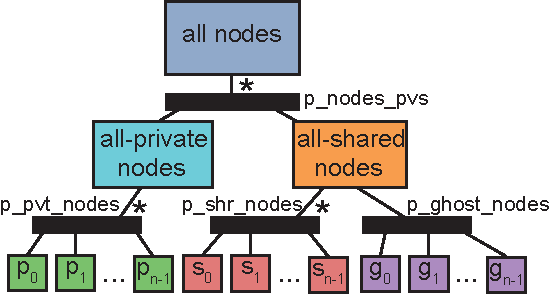
\includegraphics[scale=0.48]{figs/CircuitPartition.pdf}
}

  \subfigure[$p\_nodes\_pvs$]{
\label{sfig:part_fig:pvs}
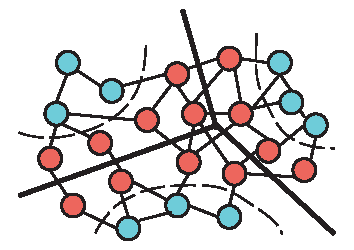
\includegraphics[scale=0.67]{figs/Private_vs_Shared.pdf}
}
  \subfigure[$p_i$]{
\label{sfig:part_fig:p_i}
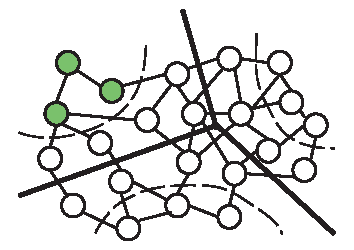
\includegraphics[scale=0.67]{figs/Private_Local.pdf}
}
  \subfigure[$s_i$]{
\label{sfig:part_fig:s_i}
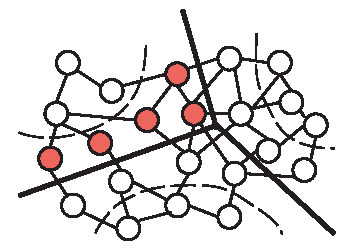
\includegraphics[scale=0.67]{figs/Shared_Local.pdf}
}
  \subfigure[$g_i$]{
\label{sfig:part_fig:g_i}
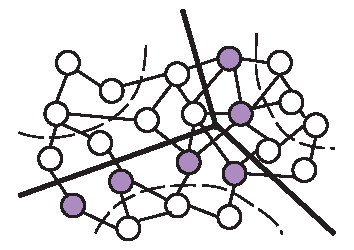
\includegraphics[scale=0.67]{figs/Ghost_Local.pdf}
}
  \label{fig:part_fig}
  \caption{Partitions of $r{\_}all{\_}nodes$.}
%  \caption[My caption
\end{figure}


\def\partitiontree{
%\draw[step=0.5,gray,very thin] (0,0) grid (8,5);

\node(top) at (3.5,4.5) { $r{\_}all{\_}nodes$ };

\node(pvsf) at (1.9,2.5) { $p{\_}nodes{\_}pvs[0]$ };
\node(pvst) at (5.1,2.5) { $p{\_}nodes{\_}pvs[1]$ };

\node(p0) at (0.7,0.5) { $p_0$ };
\node(p1) at (1.2,0.5) { $p_1$ };
\node(pd) at (1.6,0.5) { $\ldots$ };
\node(pn) at (2.3,0.5) { $p_{n-1}$ };

\node(s0) at (3.2,0.5) { $s_0$ };
\node(s1) at (3.7,0.5) { $s_1$ };
\node(sd) at (4.1,0.5) { $\ldots$ };
\node(sn) at (4.8,0.5) { $s_{n-1}$ };

\node(g0) at (5.7,0.5) { $g_0$ };
\node(g1) at (6.2,0.5) { $g_1$ };
\node(gd) at (6.6,0.5) { $\ldots$ };
\node(gn) at (7.3,0.5) { $g_{n-1}$ };

\draw[xshift=3.5cm,yshift=3.5cm] (-1,0) -- (1,0)
  node(ptf)[pos=0.25,inner sep=0] {} edge (pvsf.north)
  node[pos=0.5,anchor=south east] {$*$}
  node(ptp)[pos=0.5,inner sep=0] {} edge (top.south)
  node(ptt)[pos=0.75,inner sep=0] {} edge (pvst.north)
  ;

\draw[xshift=1.5cm,yshift=1.5cm] (-1,0) -- (1,0)
  node(pp0)[pos=0.2,inner sep=0] {} edge (p0.north)
  node(pp1)[pos=0.4,inner sep=0] {} edge (p1.north)
  node[pos=0.5,anchor=south east] {$*$}
  node(ppp)[pos=0.5,inner sep=0] {} edge (pvsf.250)
  node(ppn)[pos=0.8,inner sep=0] {} edge (pn.north)
  ;

\draw[xshift=4cm,yshift=1.5cm] (-1,0) -- (1,0)
  node(ps0)[pos=0.2,inner sep=0] {} edge (s0.north)
  node(ps1)[pos=0.4,inner sep=0] {} edge (s1.north)
  node[pos=0.5,anchor=south east] {$*$}
  node(psp)[pos=0.5,inner sep=0] {} edge (pvst.230)
  node(psn)[pos=0.8,inner sep=0] {} edge (sn.north)
  ;

\draw[xshift=6.5cm,yshift=1.5cm] (-1,0) -- (1,0)
  node(pg0)[pos=0.2,inner sep=0] {} edge (g0.north)
  node(pg1)[pos=0.4,inner sep=0] {} edge (g1.north)
  node[pos=0.5,anchor=south east] {}
  node(pgp)[pos=0.5,inner sep=0] {} edge (pvst.310)
  node(pgn)[pos=0.8,inner sep=0] {} edge (gn.north)
  ;
}

\def\partitiongraph{
%\draw[step=0.5,gray,very thin] (0,0) grid (8,5);

\node[cn,s0] (n1) at (0.77,1.27) {};
\node[cn,p0] (n2) at (1.6165,3.3865) {};
\node[cn,s0] (n3) at (2.463,2.54) {};
\node[cn,p0] (n4) at (0.8755,2.54) {};
\node[cn,p2] (n5) at (2.463,0.529) {};
\node[cn,s2] (n6) at (3.945,1.799) {};
\node[cn,s0] (n7) at (3.6275,2.963) {};
\node[cn,p2] (n8) at (4.7915,0.529) {};
\node[cn,s1] (n9) at (5.638,1.5875) {};
\node[cn,s1] (n10) at (6.6965,1.164) {};
\node[cn,s1] (n11) at (5.215,2.6455) {};
\node[cn,p1] (n12) at (6.379,2.7515) {};
\node[cn,p1] (n13) at (5.3205,3.598) {};
\node[cn,s1,g0] (n14) at (4.1565,4.1275) {};
\node[cn,s0] (n15) at (2.8865,3.81) {};
\node[cn,p0] (n16) at (0.77,4.1275) {};
\node[cn,s2,g0] (n17) at (1.405,0.423) {};
\node[cn,p1] (n18) at (6.379,4.0215) {};
\node[cn,s2,g0] (n19) at (2.7805,1.4815) {};
\node[cn,s0] (n20) at (1.7225,1.799) {};
\node[cn,p2] (n21) at (3.733,0.7405) {};
\node[cn,s2] (n22) at (5.85,0.635) {};

\draw (n16) to (n2);
\draw (n16) to (n4);
\draw (n5) to (n21);
\draw (n21) to (n8);
\draw (n12) to (n13) to (n18) to (n12);


\draw[p2s] (n1) to (n4) to (n20);
\draw[p2s] (n4) to (n3) to (n15) to (n2);
\draw[p2s] (n15) to (n7);

\draw[p2s] (n14) to (n13) to (n11) to (n9) to (n12) to (n10);

\draw[p2s] (n17) to (n19) to (n5);
\draw[p2s] (n19) to (n6) to (n8) to (n22);

\draw[s2s] (n1) to (n17);
\draw[s2s] (n20) to (n19) to (n3);
\draw[s2s] (n15) to (n14) to (n7);
\draw[s2s] (n11) to (n6) to (n9) to (n22) to (n10);

\draw[thick] (0.5,0.5) to (4,2.5);
\draw[thick] (3.75,4.5) to (4,2.5);
\draw[thick] (6.5,0.5) to (4,2.5);

\draw[dashed] (0.5,1.5) .. controls (1,2) and (1.5,2.5) .. (1.9,3.1) .. controls (2,4) .. (1.75,4.5);
\draw[dashed] (5.25,4.5) .. controls (4.75,3.5) .. (5.25,3.25) .. controls (6,3) .. (6,2.5) .. controls (6,2.25) .. (7,2.5);
\draw[dashed] (2,0.25) .. controls (2.25,1) .. (3.5,1.1) .. controls (5,1.25) .. (5.5,0.25);
}

\begin{figure}[t]
  \centering
\subfigure[Node region tree.]{
\label{sfig:part_fig:tree}
%\begin{tikzpicture}[scale=0.8]
%\partitiontree
%\end{tikzpicture}
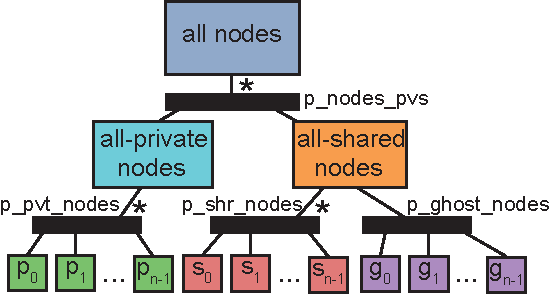
\includegraphics[scale=0.48]{figs/CircuitPartition.pdf}
}

  \subfigure[$p\_nodes\_pvs$]{
\label{sfig:part_fig:pvs}
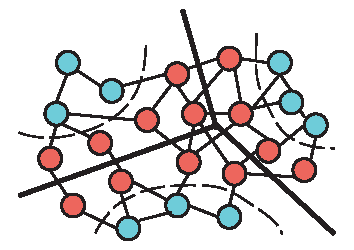
\includegraphics[scale=0.67]{figs/Private_vs_Shared.pdf}
}
  \subfigure[$p_i$]{
\label{sfig:part_fig:p_i}
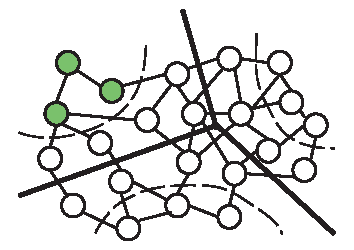
\includegraphics[scale=0.67]{figs/Private_Local.pdf}
}
  \subfigure[$s_i$]{
\label{sfig:part_fig:s_i}
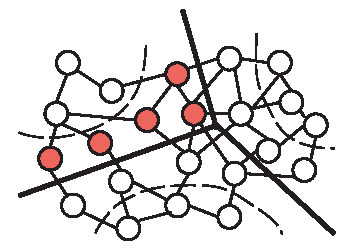
\includegraphics[scale=0.67]{figs/Shared_Local.pdf}
}
  \subfigure[$g_i$]{
\label{sfig:part_fig:g_i}
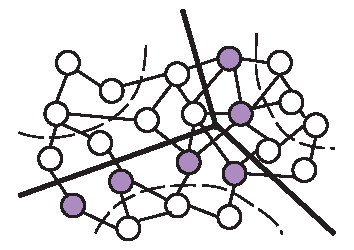
\includegraphics[scale=0.67]{figs/Ghost_Local.pdf}
}
  \label{fig:part_fig}
  \caption{Partitions of $r{\_}all{\_}nodes$.}
%  \caption[My caption
\end{figure}

\section{The Software Out-of-Order Processor}
\label{sec:soop}

There are two major challenges in implementing an efficient task
scheduler for Legion:
\begin{itemize}
\item  For correctness, Legion must guarantee that every pair of {\em dependent} tasks is executed 
in sequential order.

\item Legion must deal with and, to
  the extent possible, hide the extremely long latencies associated
  with machines that have both distributed memory and many levels of
  memory hierarchy.
\end{itemize}
We use three techniques to deal with these problems:
\begin{itemize}
\item Nested tasks (subtasks) enjoy an isolation property that allows Legion
to avoid comparing all pairs of tasks for dependences.
Specifically, the only tasks that need to be checked for dependences 
are the immediate subtasks of a common
parent task (see Section~\ref{sec:exec}).

\item Legion uses a {\em deferred execution model} that decouples the issuing
of operations from when operations are performed.  Issued operations wait for other operations on
which they are dependent to complete before executing.  For example, Legion may issue a copy
operation to move the results of a task $a$ to the place where a task $b$ will take the copied data as
an argument.  Tasks $a$ and $b$ and the copy can all be issued, but the copy will not start until
task $a$ completes and task $b$ will not start until the copy completes.

\item Legion uses a {\em  software out-of-order processor}, or SOOP, to schedule tasks.  The SOOP 
is distributed and concurrent, and also extracts nested parallelism from subtasks.
\end{itemize}
Legion's SOOP has a five stage pipeline that  decouples the management of resources from actual
task execution.  The five stages are: dependence analysis (Section~\ref{sec:dep}),
distribution (Section~\ref{sec:dist}),
mapping (Section~\ref{sec:map}),
execution (Section~\ref{sec:exec}),
and clean-up (Section~\ref{sec:clean}).
We discuss each in turn.

\usetikzlibrary{calc}
\begin{figure*}[t]
  \centering
  \subfigure[mapping of $cnc_0$ task]{
    \label{sfig:mapping_fig:cnc}
    \tiny
    \begin{tikzpicture}[scale=0.7]
      \partitiontree
      \node(cnc_p0)[very thick,draw,fill=white] at (0.45,0.30) {\tiny $cnc_0$};
      \node(cnc_g0)[very thick,draw,fill=white] at (5.45,0.30) {\tiny $cnc_0$};
      \node(def_top)[very thin,draw,fill=white] at (3.3,4.35) {\tiny ~~---~~};
      \draw[very thick] ($ (top.south)!.5!(ptp.center) $) circle (2pt);
      \draw[very thick] ($ (pvsf.north)!.5!(ptf.center) $) circle (2pt);
      \draw[very thick] ($ (pvsf.250)!.5!(ppp.center) $) circle (2pt);
      \draw[very thick] ($ (p0.north)!.5!(pp0.center) $) circle (2pt);
      \draw[very thick] ($ (pvst.north)!.5!(ptt.center) $) circle (2pt);
      \draw[very thick] ($ (pvst.310)!.5!(pgp.center) $) circle (2pt);
      \draw[very thick] ($ (g0.north)!.5!(pg0.center) $) circle (2pt);
      \draw[very thick,->] (def_top) to [bend right=45] (cnc_p0);
      \draw[very thick,->] (def_top) to [bend left=45] (cnc_g0);
    \end{tikzpicture}
  }
  \subfigure[mapping of $dc_0$ task]{
    \label{sfig:mapping_fig:dc}
    \tiny
    \begin{tikzpicture}[scale=0.7]
      \partitiontree
      %\node(cnc_p0)[very thick,draw,fill=white] at (0.45,0.30) {\tiny $\begin{array}{c}\cancel{cnc_0} \\ dc_0\end{array}$};
      \node(cnc_pn)[very thin,draw,fill=white] at (2.25,0.30) {\tiny $cnc_{n-1}$};
      \node(cnc_p1)[very thin,draw,fill=white] at (1.25,0.30) {\tiny $cnc_1$};
      \node(dc_p0)[very thick,draw,fill=white] at (0.45,0.30) 
{\tiny
$\begin{array}{@{}c@{}}
\cancel{cnc_0} \\
dc_0
\end{array}$};
      \node(cnc_gn)[very thin,draw,fill=white] at (7.25,0.30) {\tiny $cnc_{n-1}$};
      \node(cnc_g1)[very thin,draw,fill=white] at (6.25,0.30) {\tiny $cnc_1$};
      \node(cnc_g0)[very thin,draw,fill=white] at (5.45,0.30) {\tiny $cnc_0$};
      \node(dc_g0)[very thick,draw,fill=white] at (5.45,0.75) {\tiny $dc_0$};
      \draw[very thick,->] (cnc_g0.west) to [bend left=70] (dc_g0.west);
      \draw[very thick] ($ (cnc_g0.center) - (0.25,0.25) $) -- ++(0.5,0.5);
      \draw[very thick] ($ (cnc_g0.center) - (0.25,-0.25) $) -- ++(0.5,-0.5);
      \node(def_top)[very thin,draw,fill=white] at (3.3,4.35) {\tiny ~~---~~};
      \draw[very thin] ($ (top.south)!.5!(ptp.center) $) circle (2pt);
      \draw[very thin] ($ (pvsf.north)!.5!(ptf.center) $) circle (2pt);
      \draw[very thin] ($ (pvsf.250)!.5!(ppp.center) $) circle (2pt);
      \draw[very thin] ($ (p0.north)!.5!(pp0.center) $) circle (2pt);
      \draw[very thin] ($ (p1.north)!.5!(pp1.center) $) circle (2pt);
      \draw[very thin] ($ (pn.north)!.5!(ppn.center) $) circle (2pt);
      \draw[very thin] ($ (pvst.north)!.5!(ptt.center) $) circle (2pt);
      \draw[very thin] ($ (pvst.310)!.5!(pgp.center) $) circle (2pt);
      \draw[very thin] ($ (g0.north)!.5!(pg0.center) $) circle (2pt);
      \draw[very thin] ($ (g1.north)!.5!(pg1.center) $) circle (2pt);
      \draw[very thin] ($ (gn.north)!.5!(pgn.center) $) circle (2pt);
    \end{tikzpicture}
  }
  \subfigure[mapping of $volt_0$ task]{
    \label{sfig:mapping_fig:volt}
    \tiny
    \begin{tikzpicture}[scale=0.7]
      \partitiontree
      \node(dc_p0)[very thin,draw,fill=white] at (0.45,0.30) {\tiny $dc_0$};
      \node(dc_p1)[very thin,draw,fill=white] at (1.25,0.30) {\tiny $dc_1$};
      \node(dc_pn)[very thin,draw,fill=white] at (2.25,0.30) {\tiny $dc_{n-1}$};
      \node(dc_g0)[very thin,draw,fill=white] at (5.45,0.30) {\tiny $dc_0$};
      \node(volt_p0)[very thick,draw,fill=white] at (0.45,0.75) {\tiny $volt_0$};
      \draw[very thick,->] (dc_p0.west) to [bend left=70] (volt_p0.west);
      \draw[very thick] ($ (dc_p0.center) - (0.25,0.25) $) -- ++(0.5,0.5);
      \draw[very thick] ($ (dc_p0.center) - (0.25,-0.25) $) -- ++(0.5,-0.5);
      \draw[very thick] ($ (dc_g0.center) - (0.25,0.25) $) -- ++(0.5,0.5);
      \draw[very thick] ($ (dc_g0.center) - (0.25,-0.25) $) -- ++(0.5,-0.5);
      \node(dc_g0)[very thin,draw,fill=white] at (5.45,0.30) {\tiny $dc_0$};
      \node(dc_g1)[very thin,draw,fill=white] at (6.25,0.30) {\tiny $dc_1$};
      \node(dc_gn)[very thin,draw,fill=white] at (7.25,0.30) {\tiny $dc_{n-1}$};
      \draw[very thick] ($ (dc_g0.center) - (0.25,0.25) $) -- ++(0.5,0.5);
      \draw[very thick] ($ (dc_g0.center) - (0.25,-0.25) $) -- ++(0.5,-0.5);
      \draw[very thick] ($ (dc_g1.center) - (0.25,0.25) $) -- ++(0.5,0.5);
      \draw[very thick] ($ (dc_g1.center) - (0.25,-0.25) $) -- ++(0.5,-0.5);
      \draw[very thick] ($ (dc_gn.center) - (0.25,0.25) $) -- ++(0.5,0.5);
      \draw[very thick] ($ (dc_gn.center) - (0.25,-0.25) $) -- ++(0.5,-0.5);
      \node(def_top)[very thin,draw,fill=white] at (3.3,4.35) {\tiny ~~---~~};
      \draw[very thin] ($ (top.south)!.5!(ptp.center) $) circle (2pt);
      \draw[very thin] ($ (pvsf.north)!.5!(ptf.center) $) circle (2pt);
      \draw[very thin] ($ (pvsf.250)!.5!(ppp.center) $) circle (2pt);
      \draw[very thin] ($ (p0.north)!.5!(pp0.center) $) circle (2pt);
      \draw[very thin] ($ (p1.north)!.5!(pp1.center) $) circle (2pt);
      \draw[very thin] ($ (pn.north)!.5!(ppn.center) $) circle (2pt);
      \draw[very thin] ($ (pvst.north)!.5!(ptt.center) $) circle (2pt);
      \draw[very thin] ($ (pvst.310)!.5!(pgp.center) $) circle (2pt);
      \draw[very thin] ($ (g0.north)!.5!(pg0.center) $) circle (2pt);
      \draw[very thin] ($ (g1.north)!.5!(pg1.center) $) circle (2pt);
      \draw[very thin] ($ (gn.north)!.5!(pgn.center) $) circle (2pt);
      \draw[very thick] ($ (g0.north)!.5!(pg0.center) - (0.1,0.1) $) -- ++(0.2,0.2);
      \draw[very thick] ($ (g0.north)!.5!(pg0.center) - (0.1,-0.1) $) -- ++(0.2,-0.2);
      \draw[very thick] ($ (g1.north)!.5!(pg1.center) - (0.1,0.1) $) -- ++(0.2,0.2);
      \draw[very thick] ($ (g1.north)!.5!(pg1.center) - (0.1,-0.1) $) -- ++(0.2,-0.2);
      \draw[very thick] ($ (gn.north)!.5!(pgn.center) - (0.1,0.1) $) -- ++(0.2,0.2);
      \draw[very thick] ($ (gn.north)!.5!(pgn.center) - (0.1,-0.1) $) -- ++(0.2,-0.2);
      \draw[very thick] ($ (pvst.310)!.5!(pgp.center) - (0.1,0.1) $) -- ++(0.2,0.2);
      \draw[very thick] ($ (pvst.310)!.5!(pgp.center) - (0.1,-0.1) $) -- ++(0.2,-0.2);
      \draw[very thick] ($ (pvst.230)!.5!(psp.center) $) circle (2pt);
      \draw[very thick] ($ (s0.north)!.5!(ps0.center) $) circle (2pt);
      \node(def_pvst)[very thick,draw,fill=white] at (5.3,2.75) {\tiny ~~---~~};
      \draw[very thick,->] (dc_g0.north) to [bend right=30] (def_pvst.270);
      \draw[very thick,->] (dc_g1.north) to [bend right=30] (def_pvst.315);
      \draw[very thick,->] (dc_gn.north) to [bend right=30] (def_pvst.0);
      \node(volt_s0)[very thick,draw,fill=white] at (3.2,0.30) {\tiny $volt_0$};
      \draw[very thick,->] (def_pvst.190) to [bend right=40] (volt_s0.130);
    \end{tikzpicture}
  }
  \label{fig:mapping_fig}
  \caption{Mapping of tasks in region tree}
\end{figure*}




\subsection{Depedence Analysis}
\label{sec:dep}
{\small
\begin{tabular}{c|cccc}
             & Exclusive & Atomic   & Simultaneous & Relaxed \\
\midrule
Exclusive    & Dep & Dep & Dep & Dep \\ 
Atomic       & Dep & Same & Cont & Cont \\
Simultaneous & Dep & Cont & Same & None \\
Relaxed      & Dep & Cont & None & None \\
\end{tabular}
}

\subsection{Distribution}
\label{sec:dist}

\subsection{Mapping}
\label{sec:map}

\subsection{Execution}
\label{sec:exec}

\begin{figure}
\includegraphics[scale=0.48]{figs/CircuitMem.pdf}
\caption{Tasks and data for the circuit simulation on a cluster of GPUs.}
\end{figure}

\subsection{Clean-Up}
\label{sec:clean}


\section{Mapping}
\label{sec:mapping}

While the Legion programming model describes locality and independence information abstractly,
to run a Legion application on a machine we must make concrete decisions about
where tasks will be run and where region instances will be placed.  Instead of placing
the burden of decision making on the programming system, we introduce a programmable mapping
interface that gives a programmer total control over how these decisions are made.  Armed
with this interface, the programmer can then specify application- or machine-specific
mapping decisions that would be difficult for a general-purpose programming system to infer.
In this section we describe the general mapping interface (Section \ref{sec:mapinterface}),
our base implementation of this interface (Section \ref{sec:defmapper}), and the benefits
of creating custom mappers (Section \ref{sec:custommap}).

\subsection{Mapping Interface}
\label{sec:mapinterface}
A mapper is any object that implements the mapping interface.  The mapping interface
consists of ten function calls that the runtime will make to request direction from
the mapper about how a program should be executed.  To aid in performing the 
decisions made in these calls the mapper has access to a simple 
interface for inspecting the properties of the machine on which it is running.  This includes 
information about all the processors and their kinds (i.e. CPU,GPU), as well as the memories visible
to each processor and their latencies and bandwidths.  For brevity we only
discuss three of the mapping interface calls.

\begin{itemize}
\item {\tt select\_initial\_processor} - for each task the runtime system will
ask the mapper to which processor the task should be sent.  The mapper 
can choose to keep the task on the local processor or send it to any other processor
in the system.

\item {\tt permit\_task\_steal} - when handling a steal request from another processor
the runtime will ask the mapper to decide which tasks are allowed to be stolen.  
By always returning an empty set, the mapper can disable stealing.

\item {\tt map\_task\_region} - for each logical region requested for a task, the
runtime will query the mapper for a prioritized list of memories where a physical instance for this
task should be placed.  To aid the mapping decision the runtime provides a list of the current valid physical instances
of the logical region.  The mapper returns a list of memories in which the runtime
should attempt to either reuse or manifest a physical instance of the logical region.  The
runtime traverses this list and searches for a currently valid instance.  If none can be
found, it attempts to allocate a physical instance and then issue the necessary copies
to retrieve the valid data.  If both options fail, it moves on to the next memory in the list.
\end{itemize}

There are two very elegant properties of this mapping interface.  The first property is
that all decisions made by a mapper are orthogonal to the correctness of the program and can only 
impact performance.  Regardless of where a mapper chooses to place a task or map a region, 
the runtime will always schedule tasks and copies in accordance with the privileges and 
coherence properties specified in the Legion program.  Therefore when writing an application
in Legion, a programmer can begin by using the default mapper and later optimize his program
by creating a custom mapper and gradually refining its mapping decisions.

The second useful property of the mapping interface is that it isolates machine-specific decisions
to a specific module of code.  As a result, Legion programs are highly
portable.  To port a Legion program to a new architecture, a programmer only has to
implement a new mapper with decisions specific to the new architecture. 

\subsection{Default Mapper}
\label{sec:defmapper}
To make writing Legion applications easier, we provide a default mapper implementation that
can be used to get an application working quickly at a moderate performance level.  The 
default mapper employs a simple scheme for mapping tasks and regions.  When
{\tt select\_initial\_processor} is invoked for the default mapper, it first checks for which kind of processors
the task has variants (i.e. GPU).  If the fastest variant is for the kind of processor the mapper is managing
it will choose to keep the task local, otherwise it will send the task to the closest processor of the
fastest variant kind.

The default mapper employs a Cilk-like algorithm for task stealing\cite{CILK95}.  Tasks are kept local
to their target processor whenever possible and only moved when stolen.  Unlike Cilk, the default mapper
has the information necessary for locality-aware stealing.  When {\tt permit\_task\_steal} is called for a task, 
the default mapper inspects the logical regions for the task being stolen, and will mark that other tasks using 
the same logical regions should be stolen as well.

For calls to {\tt map\_task\_region}, the default mapper constructs a stack of memories ordered from best-to-worst
by bandwidth from the local processor.  This stack is then returned as the location of memories to be used for
mapping each region.  Note that this is a greedy algorithm that works well for the common case, but can cause some 
regions to be pulled unnecessarily close to the processor and consume precious fast memory space.  

\subsection{Custom Mappers}
\label{sec:custommap}
To optimize a Legion program or library, programmers can create one or more custom mappers.  
For each Legion task call the programmer specifies which mapper should be invoked by the runtime for
mapping that particular task.  This allows for the composition of Legion applications and libraries
each with their own custom mappers.

Each custom mapper extends the default mapper.  A programmer only has to override the functions necessary 
for creating a custom mapping.  Custom mappers can be used to create totally static mappings, 
mappings that memoize their results, or even totally dynamic mappings.  We describe examples of 
custom mappers in Section \ref{sec:exp}.





\section{Experiments}
\label{sec:exp}



\begin{figure}
{\footnotesize
\begin{tabular*}{3.5in}{l|ccc}
Cluster & Sapling & Viz & Keeneland \\
\midrule
Nodes   &   4     &  10 &  32 (120) \\
CPUs/Node & 2x Xeon 5680 & 2x Xeon 5680 & 2x Xeon 5660 \\
HyperThreading & on & off & off \\
GPUs/Node & 2x Tesla C2070 & 5x Quadro Q5000 & 3x Tesla M2090 \\
DRAM/Node & 48 GB & 24 GB & 24 GB \\
Infiniband & 2x QDR & QDR & 2x QDR \\
\end{tabular*}
}
\vspace{-2mm}
\caption{System configurations used for the experiments. \label{fig:systems}}
\vspace{-6mm}
\end{figure}

% FIXME
% This is a nice paragraph, but it doesn't belong here; perhaps in the mapping section
% if we have space.
%
%Nodes with multiple instances of different resources are challenging
%for existing programming models with flat system views (e.g., MPI).
%They must either lump resources together and ignore internal irregularities (e.g. NUMA
%in multi-socket x86 systems), or divide a single physical node into
%multiple smaller nodes, ignoring the better affinity between sockets/GPUs/etc.
%on the same node. In contrast, the machine model used by Legion is based on an
%affinity graph of CPUs and GPUs and accurately captures complex
%machine hierarchies.
%
% FIXME
%   I cut this from the above, commented-out paragraph because it was a digression. 
%  
% and either wasting or over-subscribing some resources when
%the quantities of different resources don't share a common divisor.


We evaluate the efficiency and scalability of Legion using
three applications on three clusters (see Figure~\ref{fig:systems}).  All three
clusters were Linux-based, and the Legion runtime was built using pthreads for
managing CPU threads, CUDA\cite{CUDA} for GPUs, and GASNet\cite{GASNET07} for
inter-node communication.  The RDMA features of GASNet were used to create a 
globally addressable, but relatively slow, {\em GASNet memory} that is accessible
by all nodes.
For each application, multiple problem sizes were used, and each size problem was
run on subsets of each machine ranging from the smallest (a single CPU core or GPU)
to the largest or near-largest (except Keeneland, where we limited
runs to 32 nodes to get sufficient cluster time).
By examining performance of the same size problem over progressively larger
machines, we measure Legion's strong scaling.
By increasing the problem size as well, we also measure weak scaling.

\subsection{Circuit Simulation}
\label{subsec:exp_ckt}

The first experiment we investigate is the distributed circuit simulation described in 
Section~\ref{sec:ex}.  The Legion SOOP runtime handles all of the resource allocation, 
scheduling, and data movement across the cluster of GPUs.  In particular,  
Legion's ability to efficiently move the irregularly partitioned
shared data around the system while keeping the private nodes and wires resident in
each GPU's framebuffer memory is critical to achieving good scalability.

Circuits of two different sizes were simulated.  The first had 480K wires, connecting
120K nodes.  The second is twice as large, with nearly 1M wires connecting 
250K nodes.  In addition to running these tests on varying numbers of
nodes, the number of GPUs used by the runtime was also varied.  In no case did the 
changes to nodes or number of GPUs per node require changes to the application code.

The circuit simulation has a simple application-specific mapper.  At initialization
time, the mapper queries the list of GPUs in the machine and identifies each GPU's
framebuffer memory and {\em zero-copy} memory (pinned memory that both the GPU and
CPUs in the system can access directly).  Once the circuit is partitioned, the partitions
are assigned a home GPU in round-robin fashion.  Every task related to that partition is
then sent to the home GPU, with no task stealing allowed.  
(In a well-partitioned circuit,
load imbalance is low enough that the cost of moving the private data for a piece from one
GPU to another outweighs any benefits.)

  The regions for the tasks are mapped as 
shown in Figure~\ref{fig:gpumapping}.  Wires and private node data are kept in each GPU's
framebuffer at all times.  An instance of the ``all-shared nodes'' region is placed in
GASNet memory and instances for just the shared and ghost nodes needed by each GPU
are placed into that GPU's zero-copy memory.  This enables the application kernels
to access the data as well as the necessary inter-node exchanges of data via the GASNet
memory.

\begin{figure}
\includegraphics[scale=0.48]{figs/CircuitMem.pdf}
\caption{Tasks and data for the circuit simulation on a cluster of GPUs.}
\label{fig:gpumapping}
\end{figure}

Figure~\ref{fig:ckt_speed} shows the performance of the Legion circuit simulation relative
to a hand-coded single-GPU implementation written in CUDA.  The hand-coded implementation is
able to keep the entire simulation state in fast framebuffer memory.  Each line shows the scaling of
a particular problem size as the number of nodes is varied.  Our results demonstrate
excellent strong scaling, with speedups of 39.0X for the small problem on 48 GPUs and 
62.5X for the larger problem size on 96 GPUs.  The inset in the graph shows the relative
performance for small numbers of GPUs.  On a single GPU, our Legion implementation
is within 5\% of the performance of the hand-coded simulation.

Figure~\ref{fig:ckt_overhead} shows the fraction of the overall simulation time (summed over
all nodes) spent in the application kernels compared to the various pieces of the Legion
SOOP runtime.  As the node count increases, the non-communication overhead stays relatively constant.
As expected the communication overhead grow linearly with number of nodes.

\begin{figure}
\subfigure[Circuit simulation speed relative to single-GPU implementation.]
{
\includegraphics[scale=0.4]{figs/circuit_speedups.pdf}
\makebox[0pt][r]{
\raisebox{0.25 in}{
\includegraphics[scale=0.4]{figs/circuit_speedups_zoom.pdf}
}
}
\label{fig:ckt_speed}
}

\subfigure[Overhead of circuit simulation on Keeneland with 3 GPUs/node.]
{
\includegraphics[scale=0.4]{figs/circuit_overhead.pdf}
\label{fig:ckt_overhead}
}
\vspace{-2mm}
\caption{Circuit simulation results.}
\vspace{-6mm}
\end{figure}

\subsection{Particle Simulation}
\label{subsec:exp_fluid}

Our second experiment is a port of the \emph{fluidanimate} benchmark
from the PARSEC suite\cite{bienia11benchmarking}, which does a
particle-based simulation of an incompressible fluid.  Each particle
interacts only with other nearby particles. The benchmark divides the
space in which the fluid can move into a three-dimensional array of
cells such that the range of interaction is limited to just the cells
adjacent (including diagonals) to the one a particle resides in.  The
application divides the array into {\em grids} and assigns each grid to
a thread.  Per-cell locking safely accesses particles in
cells that lie on the edge of a grid.  This fine-grained locking
scheme along with the assumption of a shared address space gives
good scaling in a multi-core processor, but rules out any attempt to run
beyond a single node.

To extend the scaling further, our port uses region partitioning to
divide the array into grids in a similar way, but avoids relying
on shared memory to handle interactions between grids.
Instead, the Legion version creates
explicit ghost copies of cells on grid boundaries and uses
those ghost cells to exchange information between the grids.

The particle simulation's mapper is very simple: it maps one grid's
tasks onto each processor and maps all that grid's regions (both
internal and ghost regions) into that processor's system memory.  The
exchange of ghost cell data between processors is handled by the
Legion runtime as a ghost cell region is alternately mapped to two
different memories.

Figure~\ref{fig:fluid_single} compares the performance of the Legion
implementation against the PARSEC version, using a relatively small
problem (300K particles on a 15x21x15 array of cells).  Speedups for
both the Legion and threaded PARSEC implementations are measured 
relative to PARSEC's serial version, which eliminates all locking
operations.  Between 1 and
4 threads, the PARSEC and Legion results are nearly indistinguishable,
indicating neither the Legion runtime nor the restructuring of the
implementation to allow multi-node scaling impose any significant
overhead.
%It's possible that the use of explicit ghost cells rather than fine-grained sharing of cache lines might be a net win.  
At 8 threads and above, performance begins to vary.  Both the Legion
and PARSEC versions on Viz flatten out as they over-subscribe the 12
physical cores.  On Sapling, which has HyperThreading enabled,
deviations from linear begin sooner as the operating system's
thread placement choices begin to matter.

To measure scaling beyond a single node, three different problem sizes
were run for each of the three systems (Figure~\ref{fig:fluid_multi}).
For the smallest problem (300K particles), we observe a 20\% speedup
from 1 to 2 nodes (16 threads total), but slow
down beyond that due to communication overhead---at 4 nodes there are
twice as many ghost cells as interior grid cells.  The larger problem
sizes (2.4M and 19M particles) do much better, with scaling of up to
5.4x when going from 1 node up to 16 because of a lower
communication-to-computation ratio.

%Although the particle simulation being performed is on a regular array of cells, it turns out that the
%distribution of particles amongst the cells is very irregular.  The simulation models gravity, which points in
%the -Y direction, so the particles are clustered mostly in the lower half of the cell array.  The PARSEC
%implementation works around this imbalance by only slicing the cell array through the X and Z axes, yielding
%grids that are uniformly populated, even if the number of boundary cells (for which locks must be used) is
%increased above the minimum. MORE TEXT NEEDED HERE

\begin{figure}
\subfigure[Single-node particle simulation speed.]
{
\includegraphics[scale=0.4]{figs/fluid_singlenode.pdf}
\label{fig:fluid_single}
}

\subfigure[Multi-node scaling.]
{
\includegraphics[scale=0.4]{figs/fluid_multinode.pdf}
\label{fig:fluid_multi}
}

%\subfigure[Effect of load-balanced partitioning.]
%{
%\includegraphics[scale=0.4]{figs/fluid_balance.pdf}
%\label{fig:fluid_balance}
%}
\vspace{-2mm}
\caption{Fluid simulation results.}
\vspace{-6mm}
\end{figure}

\subsection{Adaptive Mesh Refinement}
\label{subsec:exp_amr}
Our final application is based on the third heat equation example from
the Berkeley Labs BoxLib project \cite{BoxLib}.  This application is a
three-level adaptive-mesh-refinement (AMR) code that computes a first
order stencil on a 2D mesh of cells.  
%The simulation iterates for many time steps.  
Updating the simulation for one time step consists of
three phases.  In the first phase, the boundary cells around a box at
a refined level linearly interpolate their values from the nearby
cells at the next coarsest level.  The second phase performs the
stencil computation on each cell in every level.  In the third phase,
cells at a coarser level that have been refined are restricted to the
average of the cells that they physically contain at the next finest
level of refinement.

Achieving high-performance on this application is particularly
challenging for several reasons.  First, the application has a very
high communication-to-computation ratio which, for a fixed problem
size, begins as being memory bound and with increasing node count
becomes network bound as the perimeter-to-area ratio of cell grids
increases.  Second, when choosing how to partition cells into grids,
the programmer must consider the locality between cells within a
level as well as across levels.  For
cross-level cell dependences, mapping decisions must be made at
runtime as the location of refinements are dynamically determined.
Finally, this application has parallelism both
between tasks running at the same level and tasks running across
levels, leading to complicated input-dependent data dependences.

BoxLib's implementation partitions cells within a level 
into a number of grids based on the number of nodes in the
machine and distributes one grid from each level to each node.  This
optimizes for memory bandwidth and load balance, but does not 
exploit cross-level locality between grids from
different levels of refinement.  Furthermore, BoxLib does not block
grids into sub-grids to take advantage of intra-grid locality.

Our Legion implementation performs two optimizations that allow us to
outperform BoxLib.  First, for each level of
refinement we recursively partition the logical region of cells based
on the number of nodes in the machine and the sizes of the L2 and L3 caches.
%Legion allows us to describe locality for many levels of
%the memory hierarchy instead of just at the node-level.
Our second optimization takes advantage of the cross-level locality.
We wrote an application-specific mapper that dynamically discovers
relationships between grids at different levels of refinement.  The
mapper dynamically performs intersection tests between logical regions
containing grids of different refinement levels.  If the mapper
discovers overlaps between grids from different levels, the mapper
places them on the same node in the machine.  The
mapper memoizes the intersection tests to amortize their cost.  The
mapper also dynamically load balances by distributing unconstrained
grids from the coarsest level onto under-loaded nodes.

We compared our Legion implementation against BoxLib on three
different problem sizes with a fixed number of cells per level of
refinement, but with randomly chosen refinement locations.  BoxLib
also supports OpenMP and we took their best performance from using 1,
2, 4, or 8 threads per node.  Our Legion implementation always uses
one thread per node to illustrate that in this application locality is
significantly more important than parallelism.  

Figure~\ref{fig:amr_total} gives the results.
On just one node, blocking for caches using Legion achieves up to 2.6X
speedup over BoxLib.  As node count increases, the mapper's
ability to exploit cross-level locality further increases
the performance advantage to 5.4X by reducing the total
communication costs.

As the node count increases the AMR code becomes highly dependent on
interconnect performance.  BoxLib performs much better on Keeneland
than on Viz due to the better interconnect.  
At higher node counts BoxLib
begins to catch up (see Figure~\ref{fig:amr_keeneland})
because our intra-level ghost-cell exchange 
uses GASNet memory to exchange ghost cells, requiring a
linear increase in network traffic with the number of nodes.  BoxLib
uses direct node-to-node exchanges of ghost cells, similar to
our fluid application.  A future implementation of our AMR code will
employ a similar ghost cell exchange algorithm to improve scalability.

\begin{figure}
\subfigure[Sapling results.]
{
\includegraphics[scale=0.4]{figs/Sapling_amr.pdf}
\label{fig:amr_sapling}
}

\subfigure[Viz results.]
{
\includegraphics[scale=0.4]{figs/Viz_amr.pdf}
\label{fig:amr_viz}
}

\subfigure[Keeneland results.]
{
\includegraphics[scale=0.4]{figs/Keeneland_amr.pdf}
\label{fig:amr_keeneland}
}
\vspace{-2mm}
\caption{Throughput of adaptive mesh refinement code. \label{fig:amr_total}}
\vspace{-6mm}
\end{figure}


\section{Related Work}
\label{sec:related}

MPI is the current industry standard for programming large
supercomputers\cite{MPI}.  While MPI supports asynchronous
communication operations there is no mechanism for composing
asynchronous operations.  Co-array Fortran, UPC, and Titanium
are array based languages that implement bulk-synchronous
programming models similar to MPI that allow for asynchronous
exchanges of data\cite{COARRAY_FORTRAN,UPC99,JV:Yel98}.  Like
MPI however, none of these languages allow for general composition
of asynchronous tasks, communication, and synchronization.

Both POSIX threads and OpenMP\cite{OPENMP98} are used for intra-node parallel
programming in large machines, but neither support any asynchronous
operations.  CUDA\cite{CUDA} and OpenCL\cite{Khronos:OpenCL} support
the compostition of asynchronous kernel launches and asynchronous copies
between a host node and a single GPU.  However, the only synchronization
options available in both interfaces are blocking operations on either
a stream or a work queue.  OpenCL has events similar to our interface for
expressing ordering, but has no synchronization primitive for expressing
more relaxed properties such as atomicity that can be described by a
deferred lock.  OpenCL events are not valid globally, but can only be
used with a single GPU context.

Cilk is a parallel programming model that has demonstrated the power of
asynchronous function calls\cite{CILK95}.  The Cilk {\em work-first}
principle provides a compelling theoretical argument for parallel programming
interfaces such as ours that optimize for throughput at the potential
expense of adding additional latency to the critical 
dependence path\cite{Frigo98}.

Chapel\cite{Chamberlain:Chapel} and X10\cite{X1005} are high-level parallel
programming languages that support asynchronous operations.  The constructs
introduced in these languages are higher-level and have complex 
semantics.  We view our interface as providing a potential target
for implementing these higher-level asynchronous operations in an efficient
manner similar to Legion\cite{Legion12}.

The implementation of our interface shares many similarities with large
distributed systems.  Many distributed system implement a publish/subscribe
abstraction for supporting communication that is very similar to how
we manage events and event waiters\cite{Aguilera99,Carzaniga01}.  Work has
also been done on using object oriented languages to build 
distributed systems \cite{Eugster01,Harrison97,Chang91}.  In these cases
callbacks are registered to run when event operations are triggered
from remote locations.

%
\section{Conclusion}
\label{sec:conclusion}

As large supercomputers continue to scale, the latencies associated
with common operations such as communication and synchronization will
become larger and more variable.  To effectively hide these latencies
future programming systems will need to leverage asynchronous operations
to overlap long latency operations with useful work.  We have
presented a low-level programming interface that is fully asynchronous
including a new synchronization primitive called a deferred lock.
Our interface uses events to compose asynchronous operations.  Clients
can use events to explicitly specify dependences between operations,
leaving the runtime to schedule them in a way that maximizes latency 
hiding while still obeying dependences.

We've presented an implementation of interface that is capable of running
on a large heterogeneous cluster containing both CPUs and GPUs.  We
employed micro-benchmarks to show that our implementation is efficient.
We also demonstrated that our interface is capable of supporting Legion,
an advanced high-level runtime system that fully leverages the asynchronous
features of our interface.  We showed that for three real-world applications
the asynchronous Legion implementations were between 22\% to 135\% faster than
implementations which contained blocking operations.





\bibstyle{IEEEtran}
\bibliography{bibliography}

\end{document}


